% !TEX root = ../main.tex
\section{Challenges}
\label{sec:problem}

%\iffalse
%\begin{figure}
%\centering
%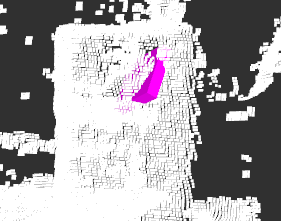
\includegraphics[width=\columnwidth]{figs/mismatch_tag}
%\caption{Close up snapshot on the rectangular prism. The physical tag is %placed on the surface of the prism but the detected tag is oriented into the %prism.}
%\label{fig:mismatch}
%\end{figure}
%\fi

In square fiducial marker detection, the pose is computed using the four corners of the tag. Since the tags are planar, it is easy to compute perspective point correspondences from the corners. This can be formalized as a specific case of pose estimation from Perspective-N-Point and it has been well studied in geometry-based Computer Vision literatures \citep{hartley2003multiple, zhang2005general}. There are numerous optimization methods such as ones proposed in \citep{dementhon1992exact} and \citep{haralick1994review} to solve this problem. In particular, in \citep{horaud1989analytic}, Horaud et al., 1989 show that there is a deterministic analytical solution to the Perspective-4-Point (P4P) problem when the points are coplanar as they are on the tag.  In practice, however, these methods are very sensitive to noise in the scene. When ARTags, Apriltags and ARToolkit systems are used in scenarios shown in Figure \ref{fig:table_clearing}, the poses of the tags are unstable even when the scene is static. Since the minimal number of perspective points are used to estimate the pose, a small variance in the corner detection process will yield estimations far from the true pose. 

We will illustrate an ambiguity effect caused by noise by using two over lapping cubes, shown in Figure \ref{fig:cube}. The overlapping face of the two cubes are interlaced but rotated by 120 degrees. However, due to perspective projection, the squares appear to be on the same plane. With low camera resolution, the overlapping squares become virtually indistinguishable. The red circular regions are the detected corners under some sensory noise. Even though the reprojection error is minimized in the 2D space using P4P optimization methods, the 3D pose can still be far off. The result of the optimization can be characterized as a bimodal distribution and a function of the the viewing angle and distance. Depending on the noise level in the scene, the optimization might converge to either one of the local minima causing the pose estimation to be unreliable. In Figure \ref{fig:simulation_results}, we ran the Apriltag pipeline on simulated tags with small Gaussian noises introduced to the image. The results show the percentage of poses that have more than $30^{\circ}$ of rotational error.